\chapter{Architettura}
\section{Introduzione}
L'architettura di \textit{Login Warrior} è basata sul design pattern architetturale$_G$ \textit{Model-View-Controller}. Il gruppo ha sviluppato un controller per ognuna delle due pagine dell'applicazione, i quali devono gestire le interazioni dell'utente con la \textit{GUI}$_G$.

 Le viste corrispondono alle pagine dell'applicazione e sono quindi due: la pagina home nella quale verrà caricato il dataset e visualizzata la lista dei grafici disponibili, e quella dove verrà effettivamente visualizzato il grafico con relativi filtri e customizzazioni.

 Il modello contiene i dati da visualizzare, che vengono presi dal file \textit{CSV} e convertiti in oggetti di tipo \textit{DataPoint} contenuti nell'oggetto \textit{Dataset}.

 Dato che viene utilizzato il servizio IndexeedDB dei browser, il gruppo ha ritenuto che questo non facesse parte di nessuno dei tre componenti sopra descritti, e quindi ha deciso di separarlo mettendolo in \textit{Services}. È comunque il controller che si occupa di gestirlo.


È stato scelto il design pattern MVC per i seguenti motivi:
\begin{itemize}
  \item Favorisce la separazione tra \textit{business logic} e \textit{presentation logic}, facendo comunicare modello e vista solo attraverso il controller;
  \item Adatto per le applicazioni che prevedono una \textit{GUI} per l'interazione con l'utente.
\end{itemize}
\section{Diagrammi delle classi}
\subsection{Model}

\begin{figure}[ht]
	\centering
	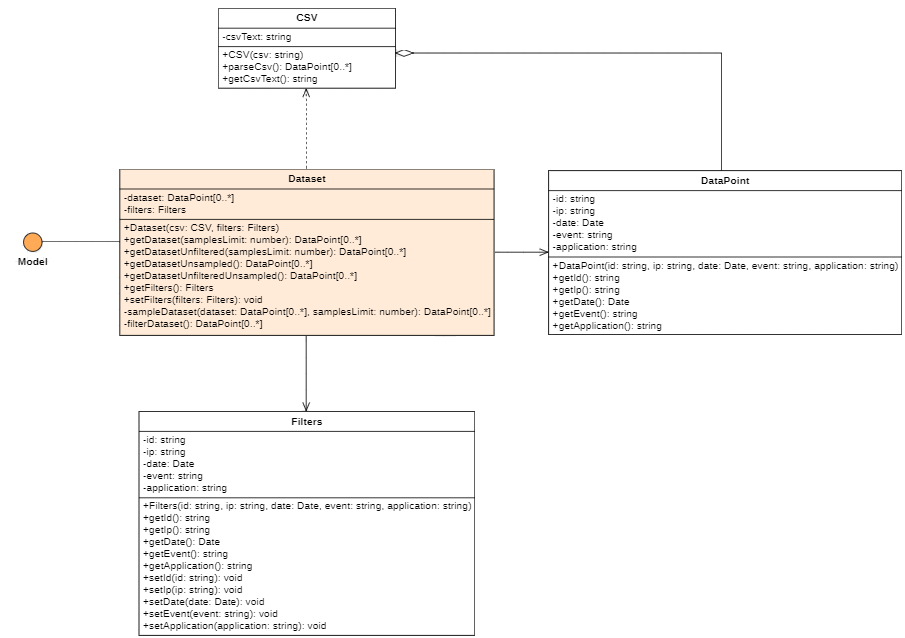
\includegraphics[width=\textwidth]{Model.png}
	\caption{Diagramma delle classi riguardanti il Model}
  \end{figure}
La funzione del modello è separare la logica dei dati dall'interfaccia.\\
Il diagramma delle classi del Model è costituito dall'interfaccia \textbf{\texttt{Model}} e dalle classi concrete \texttt{Dataset}, \texttt{Filters}, \texttt{DataPoint} e \texttt{CSV}.
Nel dettaglio la funzione delle varie componenti del model è:
\begin{itemize}
	\item \texttt{Filters}: è la classe che permette la gestione dei filtri applicati al grafico. Presenta dei metodi "get" e "set" per ogni campo dati presente, che permettono di recuperare oppure salvare i filtri applicati al grafico.
	\item \texttt{DataPoint}: è la classe che permette di salvare al suo interno le informazioni ottenute dalle tuple del file ".csv";
	\item \texttt{CSV}: è la classe che permette di salvare le informazioni presenti nel file ".csv" caricato, con il formato di array di \texttt{DataPoint};
	\item \texttt{Dataset}: è la classe più importante del Modello in quanto, oltre a salvare al suo interno tutti i filtri applicati ai grafici, salva e gestisce tutte le informazioni lette dal file ".csv" caricato.\\ La classe \texttt{Dataset} mette a disposizione differenti metodi che permettono di ottenere e salvare i filtri, salvare le informazioni dei file ".csv" e recuperare tali informazioni con delle varianti (come privarle o meno di filtri e campionature).
\end{itemize}

\subsection{View}
\begin{figure}[H]
    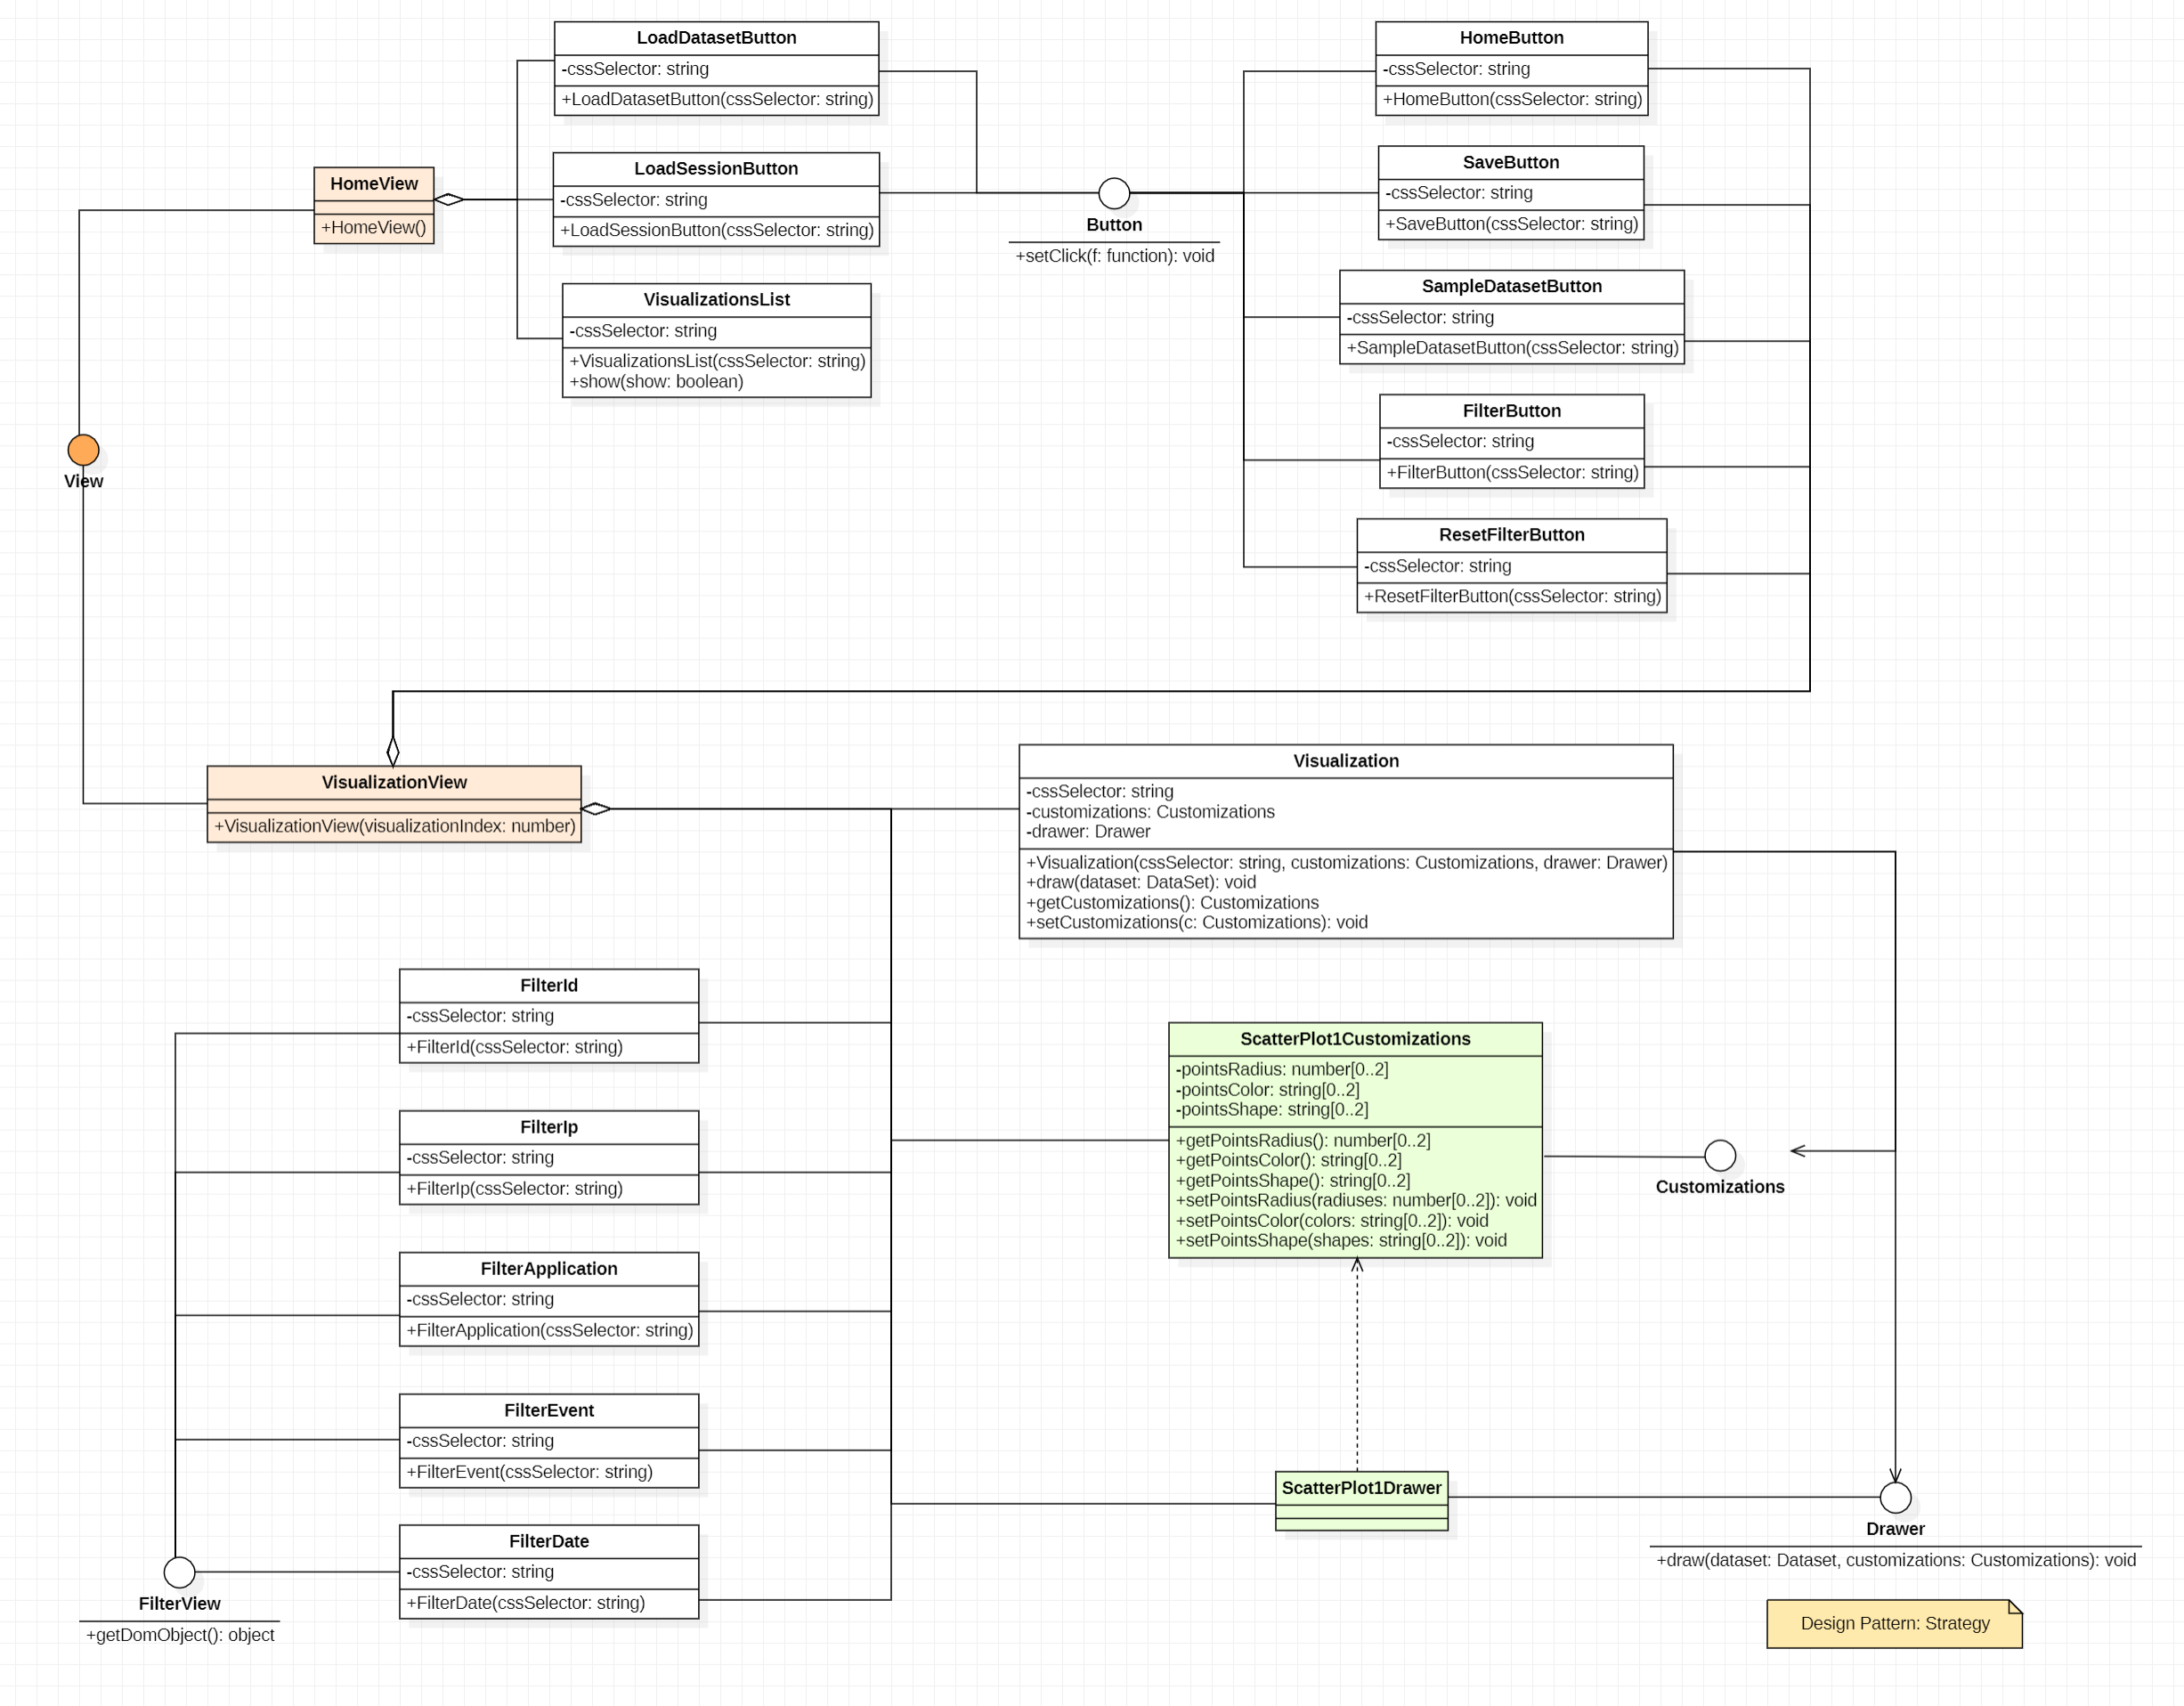
\includegraphics[width=1.0\textwidth]{vista.png}
    \caption{Diagramma delle classi riguardanti la vista}
\end{figure}
Il diagramma delle classi della vista è diviso principalmente in due parti: la classe \texttt{HomeView} e \texttt{VisualizationView} che si occupano di creare tutti gli elementi che compongono le rispettive viste e implementano un'interfaccia comune \texttt{View}.

Nella parte superiore del grafico si può notare che tutti i bottoni presenti nell'applicazione implementano l'interfaccia \texttt{Button} che mette a disposizione il metodo \texttt{setClick(f: function)} il quale conterrà l'event listener che verrà ridefinito da ogni bottone in base al suo compito.

In basso a sinistra si vede che i vari filtri impostabili implementano l'interfaccia \texttt{FilterView} che mette a disposizione il metodo \texttt{getDomObject()} il quale semplicemente restituisce l'elemento della DOM$_G$.

Come detto prima, la classe \texttt{VisualizationView} crea la classe \texttt{Visualization}, che si occupa di generare il grafico selezionato nella schermata home tramite il metodo \texttt{draw(dataset: Dataset)}, essa inoltre contiene i metodi che gestiscono le personalizzazioni dei grafici: \texttt{getCustomizations()} e \texttt{setCustomizations(c: Customizaions)}. \\Questa classe ha un riferimento alle interfacce \texttt{Drawer} e \texttt{Customizations}, dalle quali viene implementata una classe per ognuna possibile visualizzazione. In questo diagramma vengono inserite solo le classi Drawer e Customizations relative alla visualizzazione dello Scatter Plot numero 1 per renderlo più leggibile, ma come detto ogni visualizzazione ha le sue.

\subsection{Controller}
\begin{figure}[ht]
	\centering
	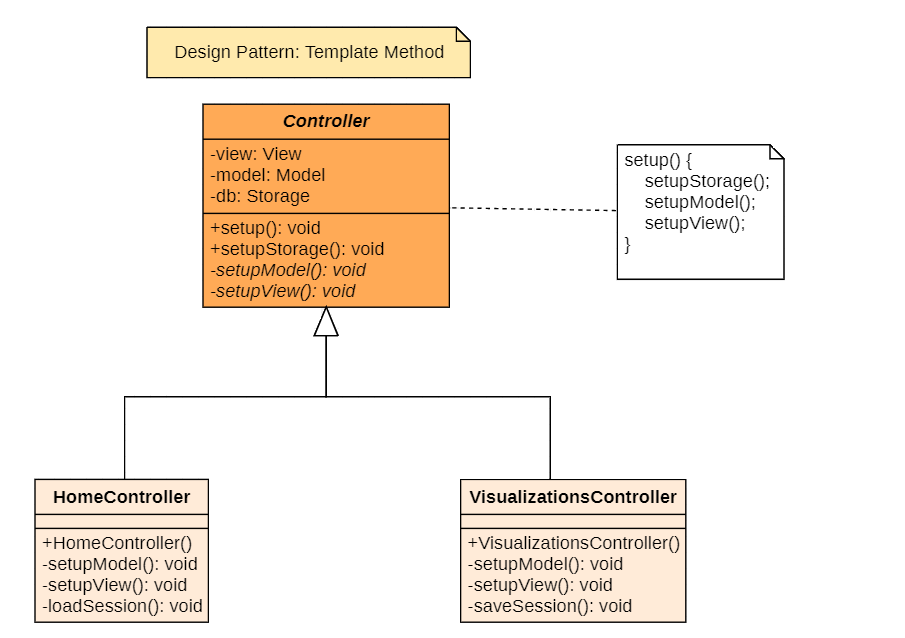
\includegraphics[width=\textwidth]{Controller.png}
	\caption{Diagramma delle classi riguardanti il Controller}
  \end{figure}
\label{controller}Il controller agisce da intermediario tra vista e modello. Ha la funzione di soddisfare le richieste poste da parte dell'utente modificando le altre due componenti.\\
Possiamo notare la presenza di una classe astratta chiamata \textbf{\texttt{Controller}} che definisce i valori e i metodi che le istanze dovranno presentare.

La scelta di usare due controller nell'applicazione è stata fatta per riuscire a gestire le pagine, con differenti funzionalità, in modo semplice e modulare permettendo una più semplice estendibilità e manutenibilità.\\
\textbf{HomeController} e \textbf{VisualizationsController} sono gli oggetti istanziabili con superclasse \textbf{\texttt{Controller}} e sono utilizzati nel seguente modo:
\begin{itemize}
	\item \textbf{HomeController}: Ha la funzione di gestire l'interazione Model-View nella scheda iniziale. Caratteristica di questa classe è la presenza del metodo privato \texttt{loadSession()} che permette il caricamento di un dataset oppure di una sessione precedentemente salvata.
	\item \textbf{VisualizationsController}: Ha la funzione di gestire l'interazione Model-View nella scheda in cui vengono visualizzati i grafici con i vari filtri. La caratteristica di questa classe è la presenza del metodo privato \texttt{saveSession()} che permette di salvare la sessione in corso con il grafico visualizzato e i filtri applicati.
\end{itemize}
Entrambe le classi precedentemente citate hanno il metodo comune \texttt{setup()} che permette l'inizializzazione della classe andando a chiamre altri tre metodi: \texttt{setupStorage()} che genera l'istanza della classe \texttt{IndexedDB}, \texttt{setupModel()} che istanzia il Modello e \texttt{setupView()} che crea la View. Completato il processo di inizializzazione l'applicazione sarà pronta a rispondere alle interazioni con l'utente.

\section{Diagrammi di sequenza}
\subsection{Caricamento dataset}
\begin{figure}[H]
	\centering
	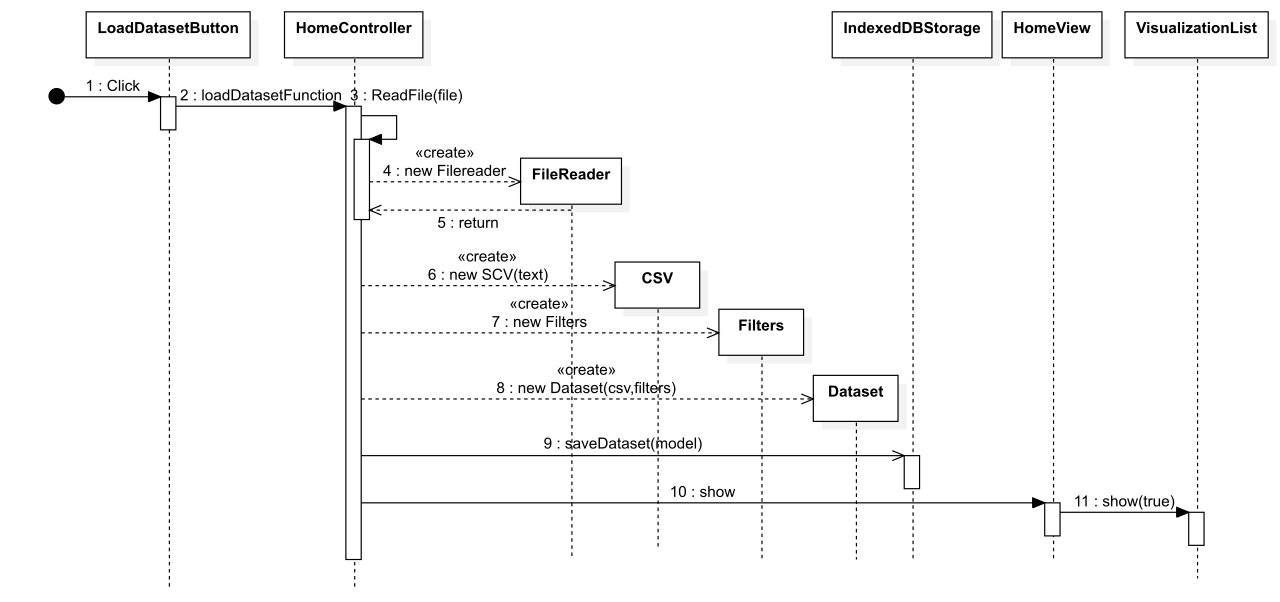
\includegraphics[width=\textwidth]{SequenceDiagramLoadDatasetButton.jpg}
	\caption{Diagramma di sequenza per il caricamento del dataset}
  \end{figure}
  La sequenza di azioni che portano al caricamento del dataset e alla conseguente visualizzazione dei vari grafici disponibili sono innescate dal "click" effettuato dall'utente sull'oggetto \texttt{LoadDatasetButton}.

Una volta cliccato \texttt{LoadDatasetButton} emetterà un segnale recepito, tramite gli EventListner, dalla classe \texttt{HomeController} che eseguirà la funzione\\ \texttt{loadDatasetFunction()}. Tale funzione chiamerà a sua volta un'altra funzione appartenente alla classe \texttt{HomeController} chiamata \texttt{ReadFile()}.
\texttt{ReadFile()} andrà semplicemente a creare un oggetto \texttt{FileReader} a cui verrà fatto leggere, sotto forma di testo, il dataset passato dall'utente.

Una volta terminata l'esecuzione della funzione \texttt{ReadFile()} continuerà l'esecuzione della funzione \texttt{LoadDatasetButton} andando a creare tre oggetti:
\texttt{CSV} a cui verrà passato come parametro attuale ciò che è stato letto da \texttt{FileReader}, \texttt{Filters} e \texttt{Dataset} a cui vengono passati come parametri attuali gli oggetti precedentemente creati \texttt{CSV} e \texttt{FileReader}.
Il passo successivo compiuto dalla funzione è chiamare il metodo \texttt{saveDataset()} dell'oggetto \texttt{IndexedDBStorage} a cui viene passato l'oggetto crato precedentemente \texttt{Dataset} con lo scopo di salvarlo nel database esterno all'applicazione.
Come ultimo passo viene chiamata la funzione \texttt{show()} dell'oggetto \texttt{VisualizationList} che permetterà la visualizzazione delle configurazioni dei grafici disponibili all'interno della HomePage.

\subsection{Nuovo campionamento}
\begin{figure}[H]
    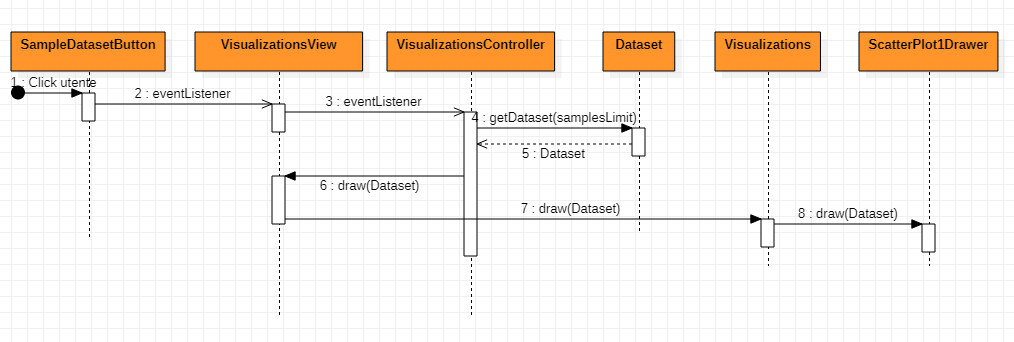
\includegraphics[width=1.0\textwidth]{sequenza_sample.png}
    \caption{Diagramma di sequenza per nuovo campionamento nel grafico \textit{ScatterPlot01}}
\end{figure}
La sequenza di azioni che portano ad eseguire un nuovo campionamento e alla conseguente visualizzazione del grafico aggiornato (in questo caso \textit{ScatterPlot01})sono innescate dal "click" effettuato dall'utente sull'oggetto \texttt{SampleDatasetButton}.\\
Una volta cliccato \texttt{SampleDatasetButton} emetterà un segnale recepito, tramite gli EventListner, dalla classe \texttt{VisualizationsController} che richiamerà la classe \texttt{Dataset} (ovvero il modello) tramite il metodo \texttt{getDataset(samplesLimit)} il quale ritornerà un nuovo insieme di oggetti \texttt{DataPoint} contenuti appunto in \texttt{Dataset}. A questo punto il controller richiamerà la funzione \texttt{draw(Dataset)} sulla classe \textit{ScatterPlot01Drawer} che genererà il nuovo grafico.


\section{Design pattern utilizzati}
\subsection{Strategy}
\begin{figure}[H]
	\centering
	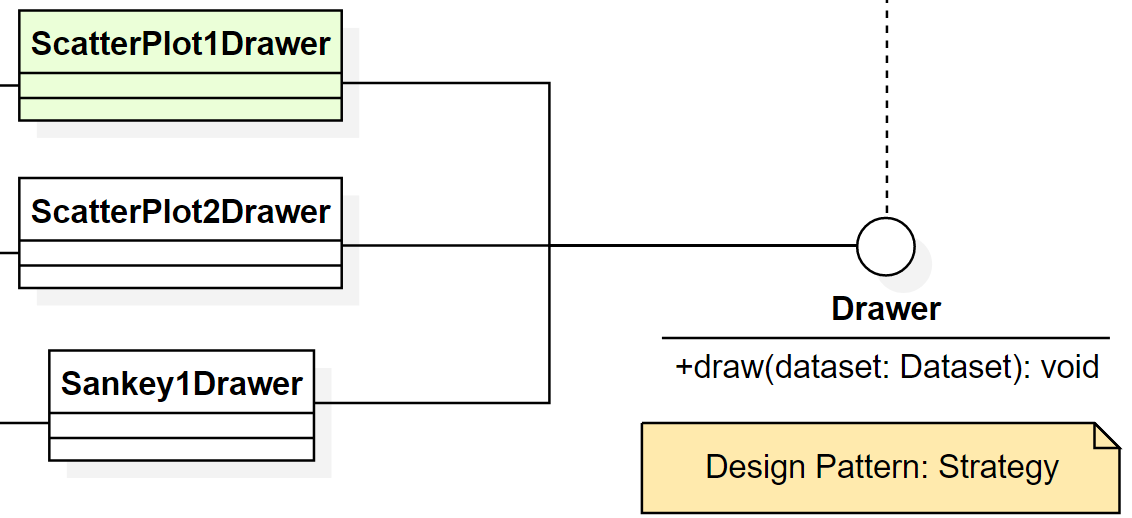
\includegraphics[width=\textwidth]{StrategyPattern.png}
	\caption{Diagramma Strategy pattern}
  \end{figure}
Il nostro gruppo ha scelto di utilizzare il pattern \textit{Strategy} per la generazione dei grafici in quanto ci serviva un algoritmo il cui fine era il medesimo, ma che sfruttasse passi differenti per la rappresentazione delle differenti viste.

Come è possibile notare dall'immagine lo \texttt{Strategy} presenta un'interfaccia chiamata \texttt{Drawer} la quale dichiara un metodo \texttt{draw(dataset:Dataset)} che sarà definito in maniera differente dalle classi che implmenteranno l'interfaccia, in questo modo sarà possibile generare grafici differenti.

Dall'immagine possiamo notare solamente tre differenti classi che implementano "Drawer" che sono \texttt{ScatterPlot1}, \texttt{ScatterPlot2} e \texttt{Sankey1Diagram}; questo è stato fatto per una questione di semplicità espositiva, in realtà ogni configurazione dei vari grafici avrà la propria classe specifica per la rappresentazione del dataset. \\

\subsection{Template method}
Il gruppo ha deciso di utilizzare il \textit{Template Method} come design pattern comportamentale nel \textit{Controller}(per il diagramma vedi \ref{controller}). \\Il motivo è che i due controller implementano un algoritmo \texttt{setup()} che ha un flusso di esecuzione comune ad entrambi: in ordine vengono eseguiti \texttt{setupStorage()}, \texttt{setupModel()} e \texttt{setupView()} che rispettivamente si occupano di creare il database, il modello e la vista. \\Ovviamente questi metodi avranno un comportamento diverso a seconda del controller in cui si trovano, ad esempio in \texttt{HomeController} il modello viene impostato dopo che l'utente ha caricato un file mentre in \texttt{VisualizationsController} il modello viene preso dal database del browser.
